% Purpose: Demonstrate accessible PGFPlots styling on a logarithmic count axis.
% Status: Draft template; human scientific and layout review pending.
% Source-of-truth: .claude/agents/latex-docxer.md (extracted plotting example).
% Origin: Hand-entered synthetic coordinates; no catalog or test fixture used.
\documentclass{article}
\usepackage[a4paper,margin=2cm]{geometry}
\usepackage{pgfplots}
\pgfplotsset{compat=1.18}

\begin{document}
\section*{Illustrative synthetic frequency--magnitude plot}

The symbol $M_L$ denotes an illustrative local-magnitude coordinate
(dimensionless); the ordinate is a synthetic cumulative count.

\begin{figure}[htbp]
  \centering
  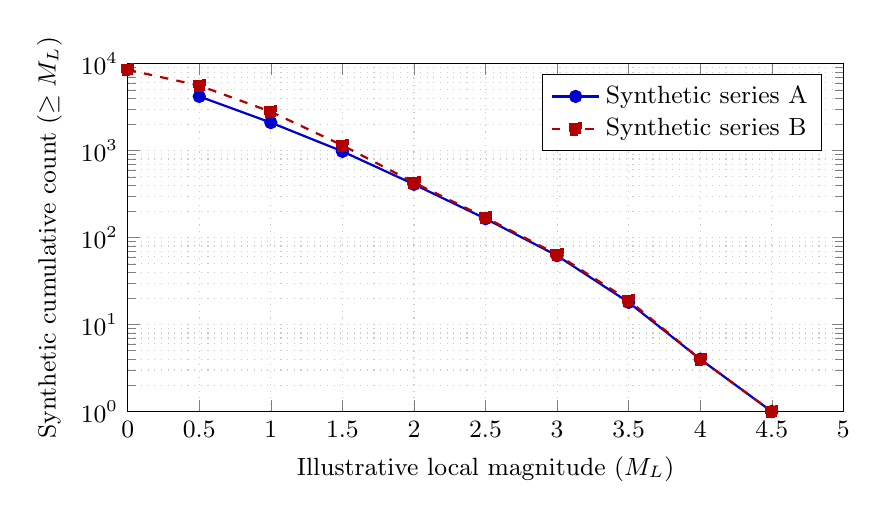
\begin{tikzpicture}
    \begin{axis}[
      width=0.88\linewidth,height=6cm,
      xlabel={Illustrative local magnitude ($M_L$)},
      ylabel={Synthetic cumulative count ($\ge M_L$)},
      xmin=0,xmax=5,ymin=1,ymax=10000,ymode=log,
      legend pos=north east,legend cell align={left},
      font=\small,grid=both,grid style={dotted,gray!40}
    ]
      \addplot[thick,color=blue!80!black,mark=*] coordinates {
        (0.5,4200) (1.0,2100) (1.5,980) (2.0,410) (2.5,165)
        (3.0,62) (3.5,18) (4.0,4) (4.5,1)
      };
      \addlegendentry{Synthetic series A}
      \addplot[
        thick,color=red!70!black,dashed,mark=square*
      ] coordinates {
        (0.0,8500) (0.5,5600) (1.0,2800) (1.5,1150) (2.0,430)
        (2.5,170) (3.0,64) (3.5,19) (4.0,4) (4.5,1)
      };
      \addlegendentry{Synthetic series B}
    \end{axis}
  \end{tikzpicture}
  \caption{Illustrative frequency--magnitude curves with distinct strokes
    and markers. The supplied counts differ at low magnitudes, but this
    is not evidence of improved detection sensitivity. Coordinates are
    hand-entered synthetic values, not catalog measurements or benchmark
    fixtures: A covers $M_L=0.5$--$4.5$ with 4200 counts at its lower cutoff,
    while B covers $0.0$--$4.5$ with 8500 counts at its lower cutoff.
    Real sample coverage, calibration, completeness, and uncertainty
    have not been evaluated.}
  \label{fig:synthetic-frequency-magnitude}
\end{figure}
\end{document}
